%%%% Better Poster latex template example v1.0 (2019/04/04)
%%%% GNU General Public License v3.0
%%%% Rafael Bailo
%%%% https://github.com/rafaelbailo/betterposter-latex-template
%%%% 
%%%% Original design from Mike Morrison
%%%% https://twitter.com/mikemorrison

\documentclass[]{betterposter}
\geometry{paperwidth=39in,paperheight=39in}
%%%% Uncomment the following commands to customise the format


%% Setting the width of columns
% Left column
\setlength{\leftbarwidth}{0.25\paperwidth}
% Right column
%\setlength{\rightbarwidth}{0.25\paperwidth}

%% Setting the column margins
% Horizontal margin
%\setlength{\columnmarginvertical}{0.0002\paperheight}
% Vertical margin
\setlength{\columnmarginhorizontal}{0.01\paperheight}
% Horizontal margin for the main column
\setlength{\maincolumnmarginvertical}{0.05\paperheight}
% Vertical margin for the main column
%\setlength{\maincolumnmarginhorizontal}{0.03\paperheight}

%% Changing font sizes
% Text font
%\renewcommand{\fontsizestandard}{\fontsize{28}{35} \selectfont}
% Main column font
%\renewcommand{\fontsizemain}{\fontsize{28}{35} \selectfont}
% Title font
%\renewcommand{\fontsizetitle}{\fontsize{28}{35} \selectfont}
% Author font
%\renewcommand{\fontsizeauthor}{\fontsize{28}{35} \selectfont}
% Section font
%\renewcommand{\fontsizesection}{\fontsize{25}{32} \selectfont}

%% Changing font sizes for a specific text segment
% Place the text inside brackets:
% {\fontsize{28}{35} \selectfont Your text goes here}

%% Changing colours
% Background of side columns
%\renewcommand{\columnbackgroundcolor}{black}
% Font of side columns
%\renewcommand{\columnfontcolor}{gray}
% Background of main column
%\renewcommand{\maincolumnbackgroundcolor}{yellow}
%\renewcommand{\maincolumnbackgroundcolor}{theory}
%\renewcommand{\maincolumnbackgroundcolor}{methods}
%\renewcommand{\maincolumnbackgroundcolor}{intervention}
% Font of main column
%\renewcommand{\maincolumnfontcolor}{gray}

\begin{document}	



\betterposter{
%%%%%%%% MAIN COLUMN

\maincolumn{
%%%% Main space
\begin{flushleft}


Higher centrality for \textbf{concentration} and \textbf{sleep} symptoms when \textbf{depression} in PTSD is accounted.
\\Results from network analysis.
\end{flushleft}

}{
%%%% Bottom space

%% QR code
\qrcode{img/qrcode.png}{img/smartphoneWhite}{
\textbf{Take a picture} to \\
download the full poster
}
{
\begin{flushright}

\includegraphics[width=0.04\textwidth]{img/twitter.png}
@orduek
\end{flushright}
}
% Smartphone icon
% Author: Freepik
% Retrieved from: https://www.flaticon.com/free-icon/smartphone_65680

%% Compact QR code (comment the previous command and uncomment this one to switch)
%\compactqrcode{img/qrcode}{
%\textbf{Take a picture} to
%\\download the full paper
%}

}

}{
%%%%%%%% LEFT COLUMN

\title{Concentration and Sleep in PTSD}
\author{Duek, Or}
\author{Hoff, Ranni}
\author{Harpaz-Rotem Ilan}
\\
\institution{Yale University School of Medicine}
\institution{National Center for PTSD}

\section{Introduction}
\begin{itemize}
\item PTSD symptomatology is still debatable
\item Past network approach studies used small/medium sample size
\item Most studies assessed PTSD symptoms alone
\item PTSD highly comorbid with depression
\end{itemize}

\section{Method}
\begin{itemize}
\item Two groups from DoD/VA administrative dataset
\item Medicated group (N=13,913)
\item Unmedicated group (N= 10,553)
\item Groups were compared in their network structure and centrality of nodes
\end{itemize}


\section{Results}
\begin{itemize}
    \item Higher centrality for sleep and concentration symptoms
    \item Anhedonia more central in unmedicated group
\end{itemize}

\begin{center}
    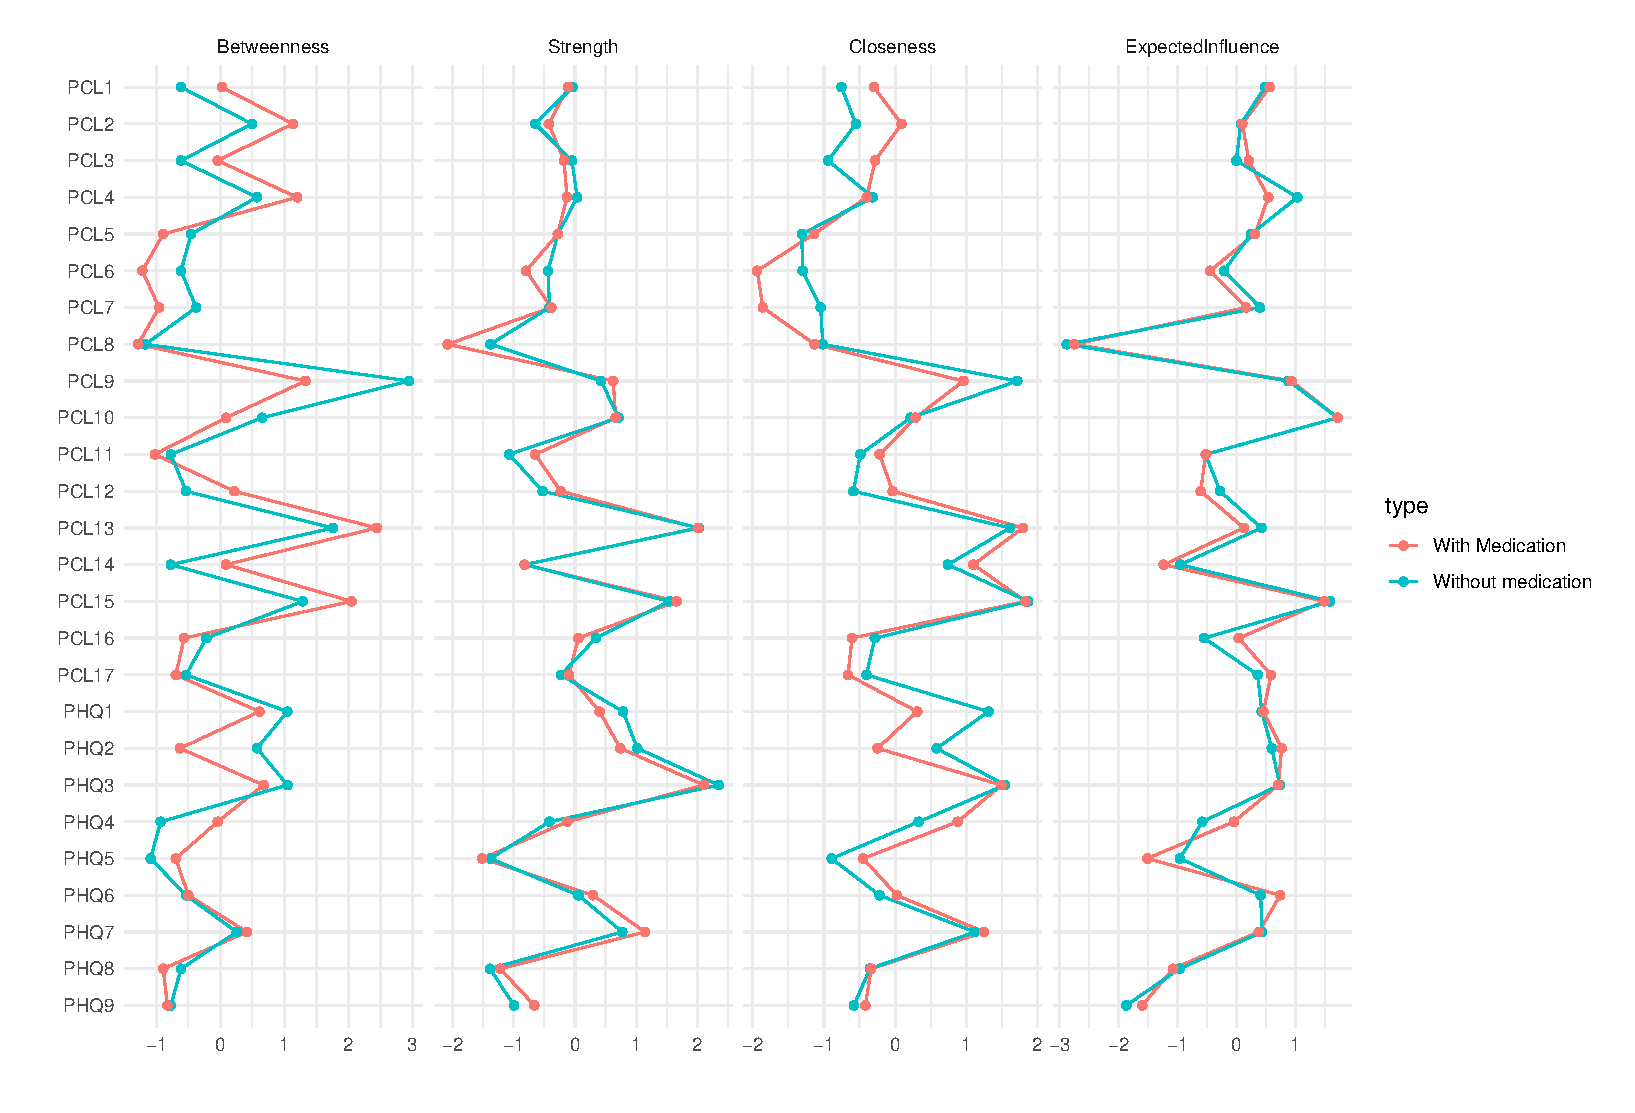
\includegraphics[width=0.95\textwidth]{img/centrality_medUnmed.eps}
\end{center}

\section{Conclusion}
\begin{itemize}
    \item Comorbidity should be taken into account
    \item Sleep and concentration are highly central in PTSD with comorbid depression
    \item Might affect our clinical intervention in future
\end{itemize}

%% This fills the space between the content and the logo
\vfill

%% Institution logo
\begin{center}



\includegraphics[width=0.3\textwidth]{img/yalesm.png}\\
\end{center}
}{
%%%%%%%% RIGHT COLUMN

\section{supplementary material}
\section{Network Graphs}
\begin{center}
% Commutative diagram with edges passing under/over
% Author: Stefan Kottwitz, http://texblog.net/
% Retrieved from: http://www.texample.net/tikz/examples/commutative-diagram/
Medicated network
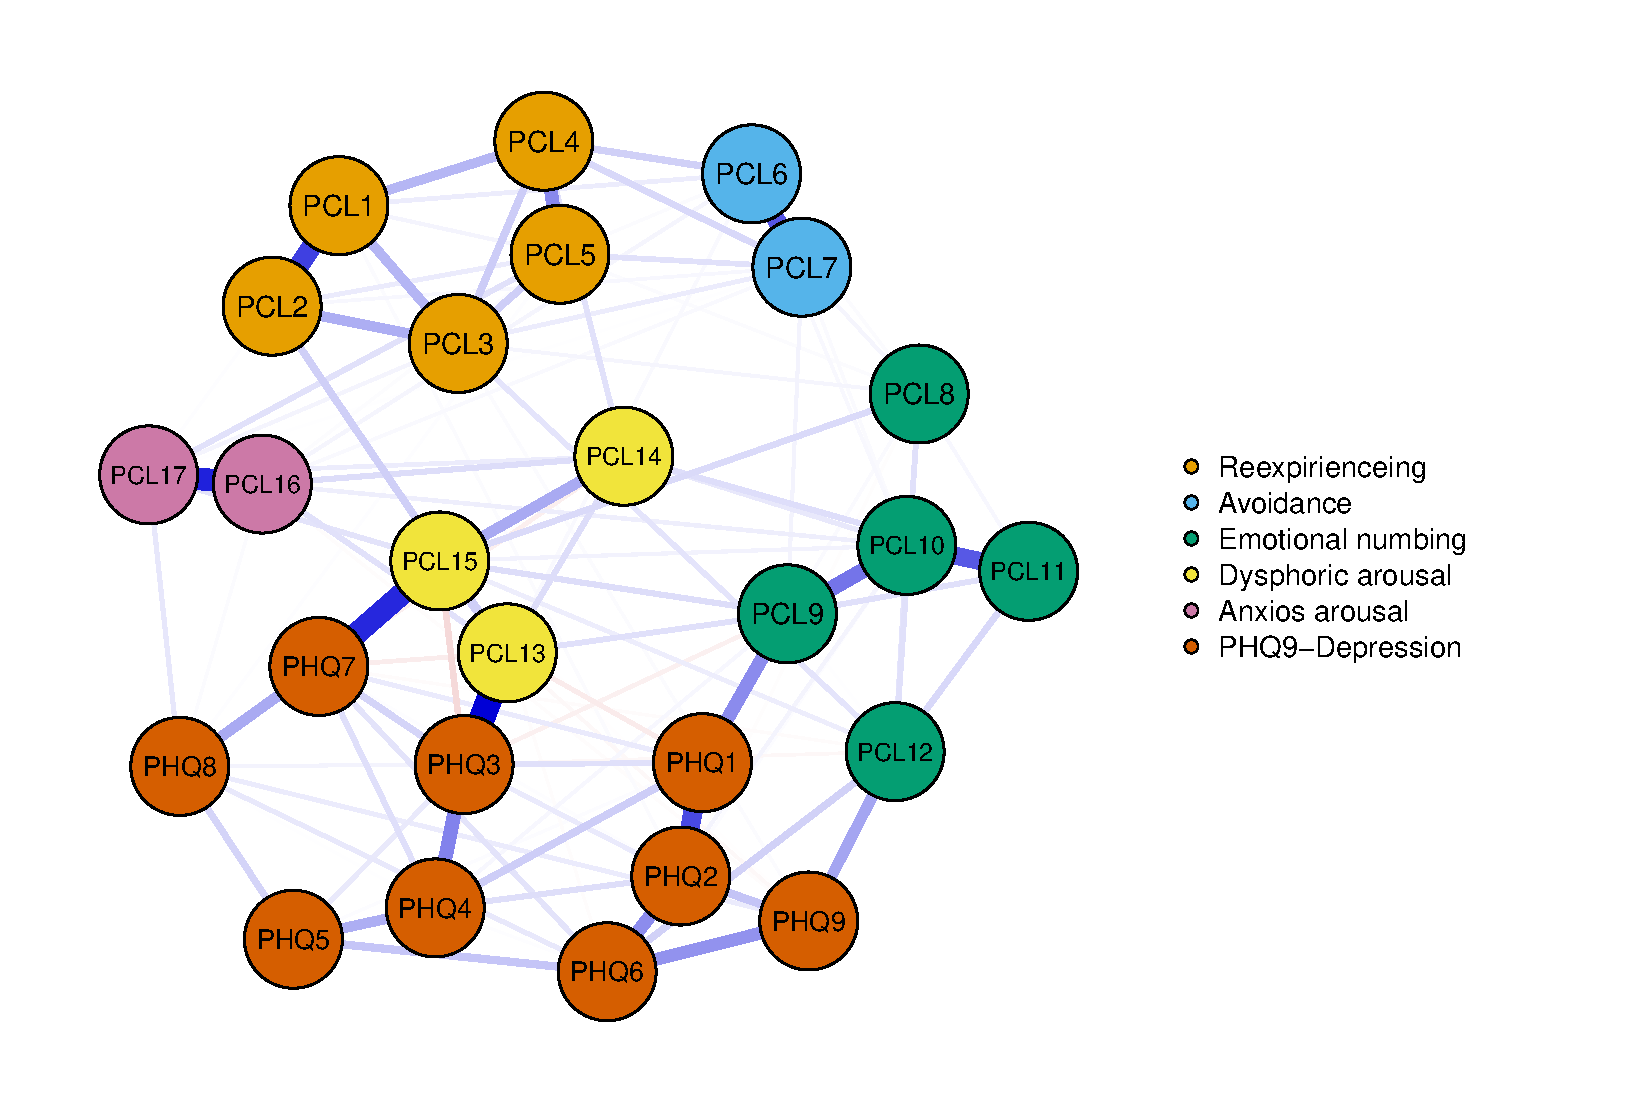
\includegraphics[width=\textwidth]{img/medicated_network.eps}
\\
Unmedicated network
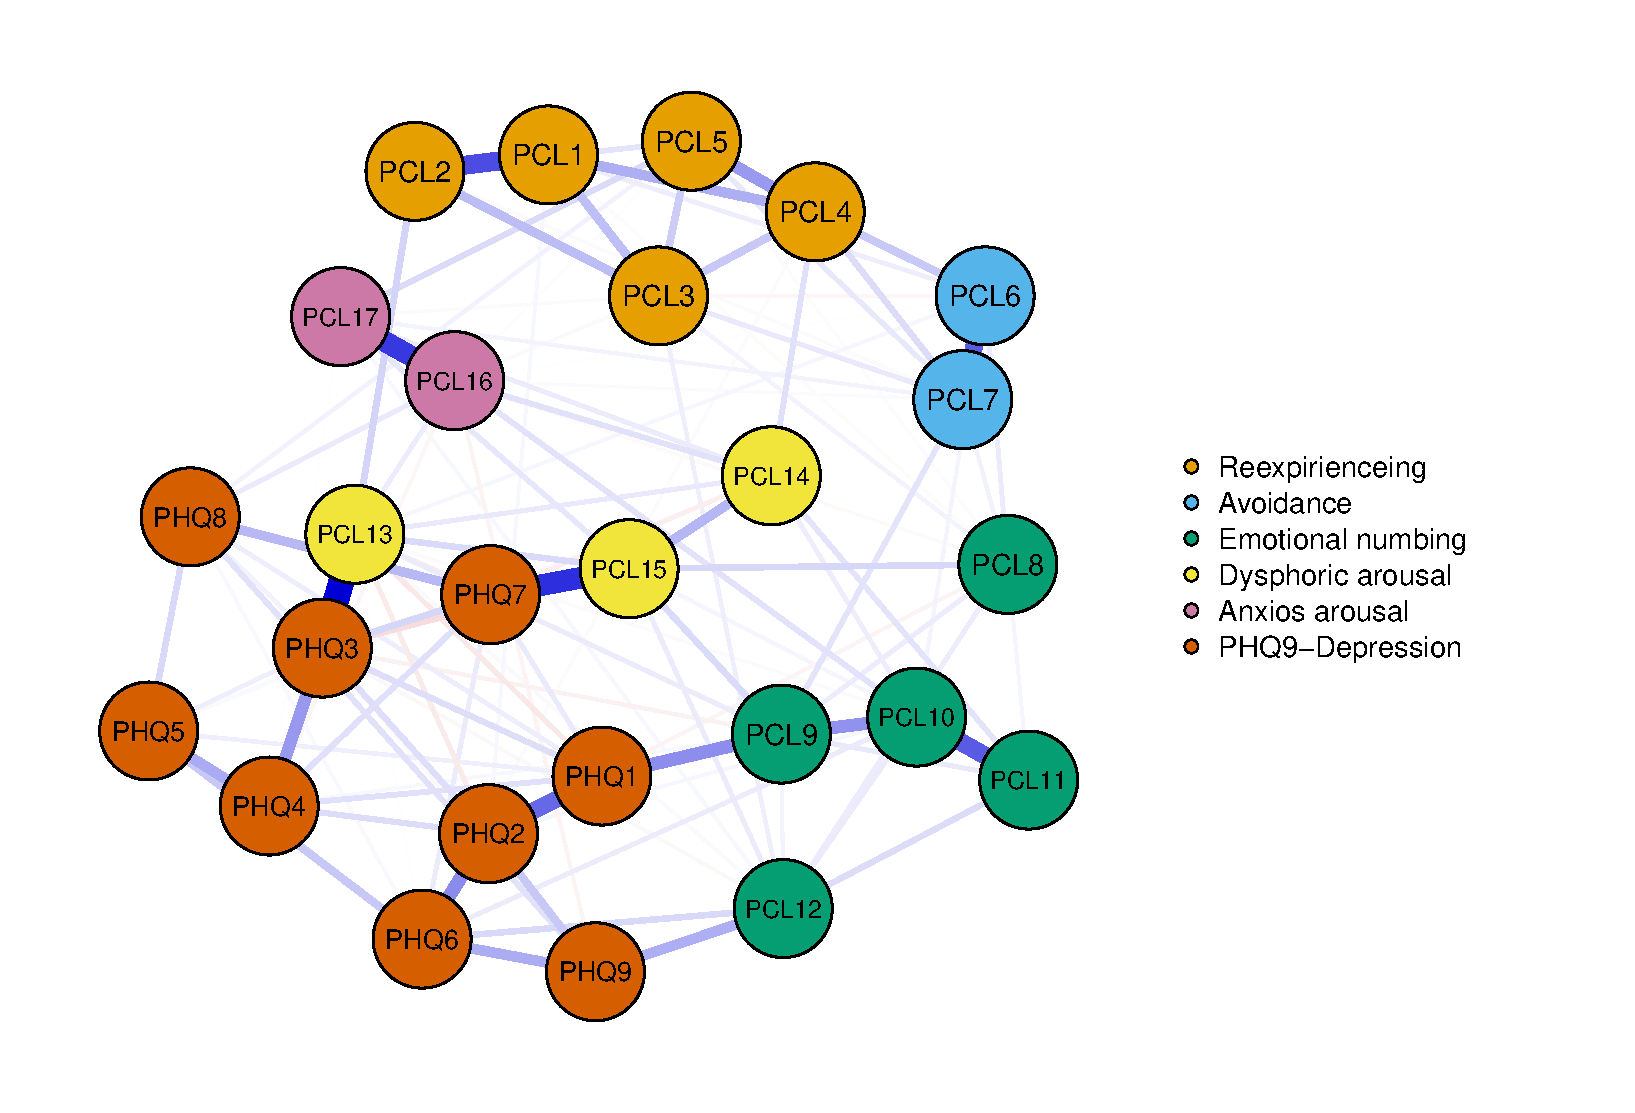
\includegraphics[width=\textwidth]{img/unmedicated_network.eps}
\end{center}

\section{More info}
\begin{itemize}
    \item Data was analyzed using R packages bootnet $^{(Epskamp \& Fried, 2018)}$
    \item As datasets are large, stability of the network is very high
    \item Network analysis is a new approach to understand symptomatology
    \item It can be used to eventually generate new understandings and better interventions
\end{itemize}

\vfill
\begin{flushright}
    

    

\includegraphics[width=0.5\textwidth]{img/NCPTSD_Logo.png}
\hfill

\includegraphics[width=0.4\textwidth]{img/Yale.png}
\end{flushright}
}

\end{document}





